\documentclass[11pt,twoside]{article}

% Official Informatica journal style (Informatica, Ljubljana, Slovenia).
\usepackage{Informat}
\usepackage[T1]{fontenc}
\usepackage[utf8]{inputenc}
\usepackage{graphicx}
\usepackage{booktabs}
\usepackage{tabularx}
\usepackage{array}
\usepackage{amsmath}
\usepackage{amssymb}
\usepackage[hidelinks]{hyperref}
\newcolumntype{L}[1]{>{\raggedright\arraybackslash}p{#1}}

% Volume, page, and DOI data are assigned by the journal after acceptance.
\def\journal{Informatica}
\def\doi{}

\usepackage[backend=biber,style=numeric,sorting=none,doi=true,url=true,isbn=false]{biblatex}
\addbibresource{refs.bib}
\renewcommand*{\bibfont}{\small}
\AtBeginBibliography{\raggedright}

\begin{document}
\raggedbottom

\title{Ski Jump Trajectory Reconstruction Using Ridge-Estimated Linear State-Space Models and Interactive Simulation}
\author{Živa Hegler$^{1}$ and Neca Camlek$^1$\\
  $^1$University of Ljubljana, Ljubljana, Slovenia\\
  \texttt{hegler.ziva0@gmail.com}, \texttt{neca.camlek@gmail.com}\\
  %$^*$Corresponding and lead author
  \AndAuthor
  Jakob Jelenčič, Marko Grobelnik and Dunja Mladenić\\
  Jožef Stefan Institute, Jamova cesta 39, 1000 Ljubljana, Slovenia\\
  \texttt{jakob.jelencic@ijs.si}, \texttt{marko.grobelnik@ijs.si},
  \texttt{dunja.mladenic@ijs.si}}
\titleodd{Ski Jump Trajectory Reconstruction Using State-Space Models}
\authoreven{Ž. Hegler et al.}
\keywords{state-space models, ski jumping, trajectory reconstruction, ridge regression, interactive simulation}
% \received{}

\abstract{We conditionally reconstruct ski-jump trajectories from measured wind and jumper-configuration profiles. Of 223 supplied Planica jumps, 203 passed quality checks. A ridge-estimated 14-state, 20-control linear state-space model ($\alpha=10$) is evaluated by jump-level leave-one-out cross-validation. With the measured initial state, mean spatial trajectory error is 1.34~m, with 95\% CI (confidence interval) 1.24--1.43~m, terminal-coordinate-distance (magnitude of over/under prediction) MAE (mean absolute error) is 1.68~m. Training-fold average-path and constant-velocity baselines yield 2.64 and 58.33~m. Timestamp defects were repaired before resampling, the 144 jumps needing no repair yield a similar 1.39~m error. An additional model with non-overlapping state and control variables recursively represents speed with seven states and 19 controls. Its trajectory error remains 1.35~m, but distance MAE rises to 4.52~m. The mean transition-matrix spectral radius is 1.0135, so both models are restricted to observed horizons. We also present a client-side application for interactive controls and three-dimensional visualization. Rather than introducing a new identification algorithm, this study evaluates established state-space methods on Planica data and implements the fitted model in an interactive application.}
\abstractSi{Predstavimo linearni model prostora stanj za rekonstrukcijo trajektorij smučarskih skokov iz Planice. Model ovrednotimo z navzkrižnim preverjanjem na 203 skokih, povprečna prostorska napaka znaša 1,34~m. Različica z ločenimi spremenljivkami stanja in vhoda doseže podobno napako poti, vendar večjo napako končne razdalje. Model je namenjen rekonstrukciji na opazovanem časovnem območju in je vključen v interaktivno spletno aplikacijo.}

\maketitle

\section{Introduction}

Ski-jump flight depends on the athlete's motion, ski orientation, hill geometry, and spatially varying wind. These quantities form a short multivariate time series rather than a single independent observation. Physics-based analyses have explained aerodynamic forces and optimized flight posture \cite{muller1996dynamics,meile2006aerodynamics,seo2004optimal}, while recent data-driven work has reconstructed trajectories or predicted jump length from wearable sensors and recorded pose sequences \cite{fang2020trajectory,schwinn2022xlength,zecha2018convolutional}. The present study investigates whether a compact linear dynamical model can reconstruct an entire measured path when its initial state and time-varying wind and posture profiles are supplied.

This study applies established state-space and ridge-regression methods to a previously unpublished Planica dataset and evaluates them with jump-level validation and a spatial path metric. A browser-based interface makes the fitted model available for interactive inspection. The work does not propose a new identification algorithm, and potential uses in safety, hill design, and competition fairness remain topics for future research rather than validated outcomes.

The study addresses four RQs (research questions):
\begin{description}
  \item[RQ1:] How accurately does a ridge-estimated linear state-space model reconstruct a held-out trajectory when its measured control profile is provided?
  \item[RQ2:] How sensitive is reconstruction to replacing the measured initial state with a mean initial state computed exclusively from the training folds?
  \item[RQ3:] How does the model compare with simple trajectory baselines, and is its learned transition matrix stable over unbounded recursion?
  \item[RQ4:] How does removing state--control overlap and recursively predicting speed affect whole-path and terminal accuracy?
\end{description}

The contributions are: (i) a fully specified 14-state, 20-control model and leakage-controlled leave-one-out evaluation, (ii) separate trajectory, endpoint, and terminal-coordinate-distance results with per-jump dispersion, (iii) an independent-vector sensitivity model that separates recursively predicted state variables from prescribed controls, and (iv) a new client-side interactive website for inspecting finite-horizon model responses. Figure~\ref{fig:architecture} summarizes the flow from the supplied measurements to the evaluated model and website.

\begin{figure}[htb]
  \centering
  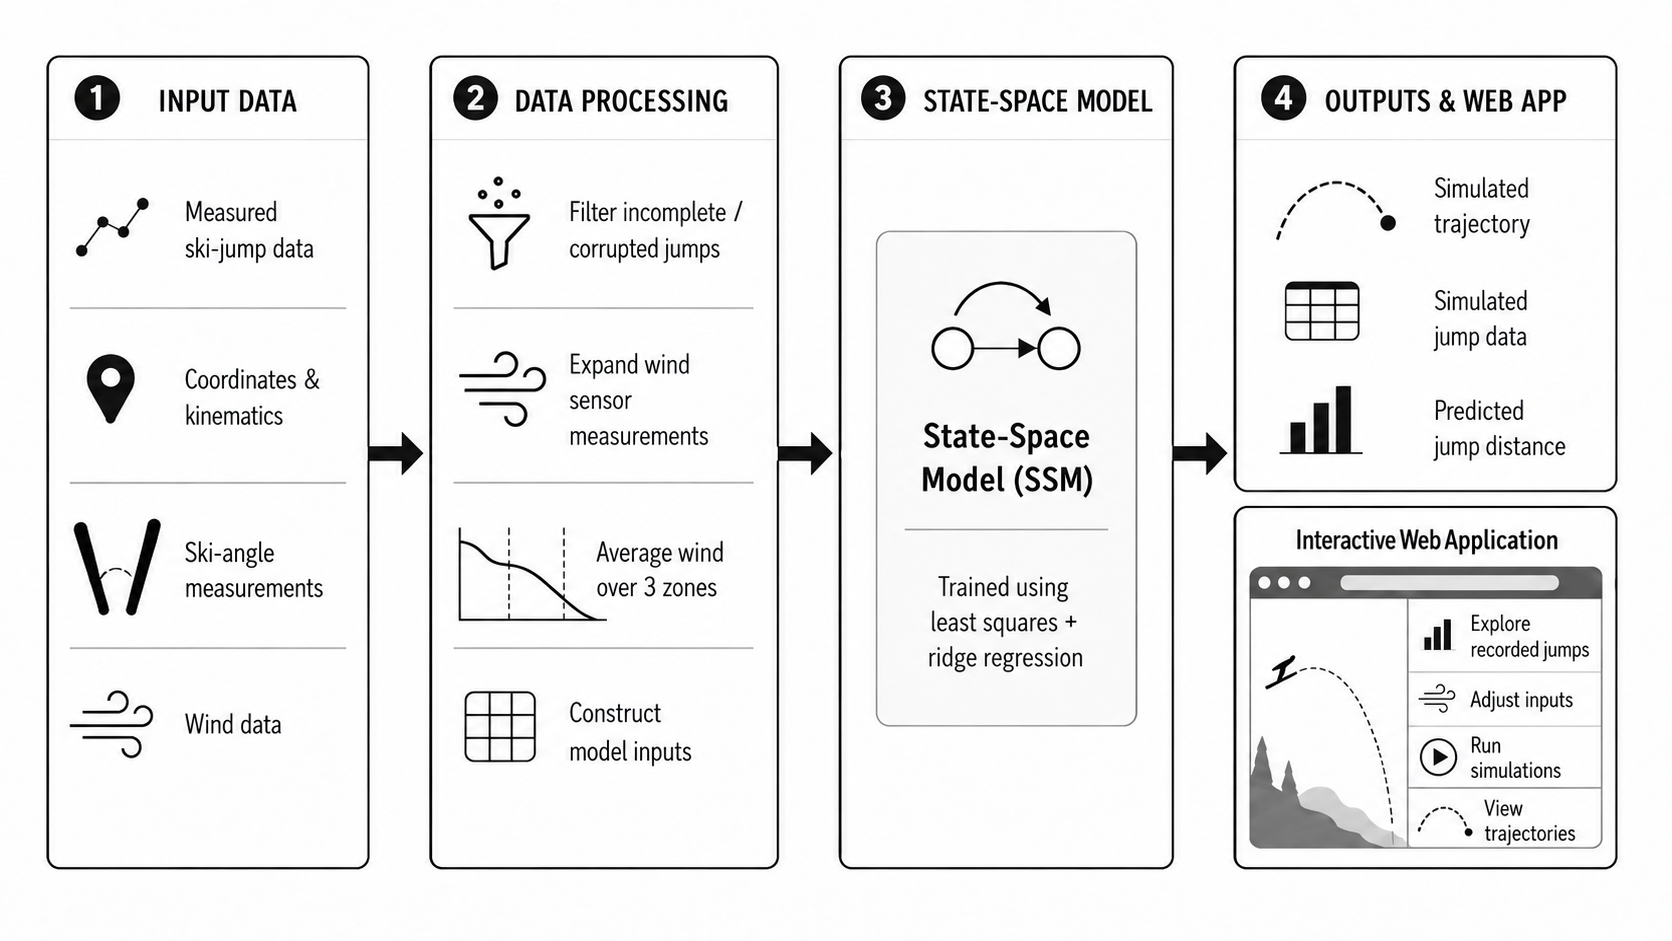
\includegraphics[width=\linewidth]{architecture.png}
  \caption{Study workflow. Raw Planica jump and wind records pass through file-level quality screening, temporal resampling, feature construction, and zone-wise wind aggregation. Ridge regression estimates the state transition and control matrices. Jump-level cross-validation evaluates held-out trajectories, while a final fit is exported as versioned JSON (JavaScript Object Notation) for the client-side website.}
  \label{fig:architecture}
\end{figure}

\section{Related Work}\label{sec:related}

\subsection{System identification and state-space models}

Linear state-space models and least-squares system identification provide an interpretable description of a dynamical system through state, input, and observation equations \cite{aoki1990state,ljung1999system,bjorck1996least}. Ridge regression stabilizes estimation with correlated predictors by adding an $L_2$ penalty \cite{hoerl1970ridge}. More formally, for a response vector $\mathbf{y}$, design matrix $\mathbf{X}$, and coefficient vector $\boldsymbol{\theta}\in\mathbb{R}^{p}$, the ridge estimator is defined by
\[
\widehat{\boldsymbol{\theta}}_{\mathrm{ridge}}
=
\operatorname*{arg\,min}_{\boldsymbol{\theta}}
\left\{
\left\lVert
\mathbf{y}-\mathbf{X}\boldsymbol{\theta}
\right\rVert_2^2
+
\alpha\left\lVert\boldsymbol{\theta}\right\rVert_2^2
\right\},
\]
where
\[
\qquad
\left\lVert\boldsymbol{\theta}\right\rVert_2^2
=
\sum_{j=1}^{p}\theta_j^2,
\]
and $\alpha\geq 0$ controls the strength of the penalty. It discourages excessively large coefficients and reduces sensitivity to correlated or noisy predictors, but usually shrinks coefficients toward zero rather than setting them exactly to zero. Nonlinear and uncertainty-aware extensions include extended and unscented Kalman filters (represent current uncertainty with a small set of possible states, passes each state through the nonlinear equations, and recombines the results) and particle methods \cite{sarkka2013bayesian}. This approximates the updated mean and uncertainty without the derivative-based linearization used by an extended Kalman filter. Our study uses the simpler deterministic linear formulation and asks whether it can reconstruct ski-jump paths from sparse distributed measurements.

\subsection{Ski-jump trajectory and length estimation}

Fang et al. reconstructed position and velocity from wearable inertial sensors with a constrained extended Rauch--Tung--Striebel smoother \cite{fang2020trajectory}. Their target is retrospective sensor fusion, whereas ours is control-conditioned path reconstruction. Link et al. introduced \textit{xLength}, which predicts final length shortly after take-off using deep networks and a substantially larger, multi-athlete dataset \cite{schwinn2022xlength}. Zecha et al. predicted multimodal dynamics from recorded pose sequences with a convolutional sequence-to-sequence model \cite{zecha2018convolutional}. These studies use different inputs and endpoints, so their published errors are not directly comparable to our full-path spatial error.

\subsection{Aerodynamic simulation, technique, and safety}

Wind-tunnel and numerical studies have quantified forces on skis and athletes \cite{seo2004aerodynamic,virmavirta2019aerodynamics,barnes2022flight}, while CFD (computational fluid dynamics) studies resolve posture-dependent flow in greater detail \cite{meile2006aerodynamics,ryu2015aerodynamic,yamamoto2022transient,hu2024unfavorable}. Physics-based simulation has been used to optimize flight technique \cite{muller2008simulation,seo2004optimal,jung2019optimization} and to study individual styles \cite{schmolzer2005individual}. Simulation studies have also examined the effects of wind on jump distance and the fairness of wind-compensation systems \cite{virmavirta2012wind,jung2018wind,jung2021windcorrigendum}. Building on a multi-body ski-jumper model, robust trajectory optimization evaluates optimized flight trajectories across plausible variations in uncertain quantities such as wind and body mass, thereby quantifying the range of possible landing positions and informing safety constraints that keep these positions within a safe landing region \cite{piprek2018multibody,piprek2018robust}. Our linear model is less physically expressive, but inexpensive to fit and suitable for real-time interaction with the limited available data.

\begin{table*}[t]
\centering
\small
\begin{tabularx}{\textwidth}{@{}L{2.7cm}L{3.0cm}L{3.1cm}L{3.0cm}>{\raggedright\arraybackslash}X@{}}
\toprule
Study & Method & Principal inputs & Output & Difference from this study \\
\midrule
Fang et al. \cite{fang2020trajectory} & Constrained extended Rauch--Tung--Striebel smoother & Wearable inertial sensors & Reconstructed trajectory & Sensor-fusion reconstruction, no interactive wind controls \\
Link et al. \cite{schwinn2022xlength} & Deep neural models & Early-flight wearable signals & Expected final length & Scalar endpoint, larger multi-venue dataset \\
Zecha et al. \cite{zecha2018convolutional} & Convolutional sequence-to-sequence model & Recorded pose sequences & Multimodal jump dynamics & Pose-sequence input and nonlinear deep model \\
Müller \cite{muller2008simulation} & Physics-based simulation & Wind-tunnel coefficients and mechanics & Simulated flight & Mechanistic rather than data-identified dynamics \\
Meile et al. \cite{meile2006aerodynamics} & Experiments and CFD & Geometry, posture, and flow & Aerodynamic field and forces & High-fidelity force analysis, not statistical path evaluation \\
This study & Ridge-estimated linear SSM (state-space model) & Initial state, zone winds, speed, and posture profiles & Full conditional trajectory and terminal-coordinate distance & --- \\
\bottomrule
\end{tabularx}
\caption{Positioning relative to representative state-space, deep-learning, and aerodynamic ski-jump studies. Numerical errors are not placed in one ranking because the studies predict different quantities from different sensors and populations.}
\label{tab:related}
\end{table*}

\section{Data and Preprocessing}\label{sec:data}

\subsection{Dataset and quality screening}

The Ski Association of Slovenia supplied the jump records from men's training at the ski flying hill (Letalnica bratov Gorišek) in Planica during the March 2024 event. Project documentation records 223 originally supplied CSV (comma-separated values) files that use semicolon delimiters. The present reproducibility package begins after initial screening and contains 203 of them. Each file represents one jump and contains position, height above ground, relative time, Cartesian coordinates, seven ski-orientation angles, three speed variables, and a compound field with measurements from 12 wind sensors. The athlete in every supplied filename is anonymized and consequently, neither the number of athletes nor model performance for each athlete separately can be determined from the available material. This is reported as a dataset limitation rather than treated as a single-athlete dataset.

Nineteen files were removed before the current 203-file folder was assembled. The documented screening criteria were (i) one or more empty columns, (ii) successive $X$, $Y$, or $Z$ values implying a physically impossible displacement across the hill within one sampling interval (a coordinate ``teleportation'') or (iii) measurements stoping mid jump. The retained records contain 88--164 samples (median 137, mean 136.62), corresponding to 4.35--8.15~s (median 6.80~s) at the 0.05~s interval. The derived terminal-coordinate distance $\sqrt{X_{\mathrm{end}}^2+Z_{\mathrm{end}}^2}$ ranges from 117.78 to 242.35~m (median 208.74~m, mean $205.54\pm21.37$~m).

These criteria distinguish unusable files from isolated missing cells. After file screening and temporal resampling, 21 missing roll-angle cells remained in four otherwise valid sequences: 18 left-roll values and three right-roll values. They were imputed by forward fill followed by backward fill. All 21 gaps were internal, so forward fill supplied the values and the backward-fill fallback did not alter them. No wind, coordinate, speed, opening-angle, yaw, or stalling-angle value required this imputation, and no rejected file was restored by it.

\subsection{Coordinate, wind, and temporal processing}\label{sec:processing}

The coordinate origin is the take-off point. $X$ follows the hill, $Y$ is lateral, and $Z$ is vertical. Angles are opening angle and left/right roll, yaw, and stalling angles, the definitions follow standard ski-jump aerodynamics, describing an exact position of skies in space \cite{muller2008performance,virmavirta2019aerodynamics}. The compound wind column was split into sensor and feature fields. For each of three hill zones (sensors 1--4, 5--8, and 9--12), we average speed, tangential wind, crosswind, and turbulence, producing 12 wind controls. The separate wind timestamp is not used as a predictor. The supplied records repeat the most recent wind reading between sensor updates, the fixed-interval resampling then linearly interpolates all numeric columns, including wind. 

Although the source files contain approximately metre-spaced position records, the dynamical recurrence is evaluated in time. Full timestamps in ISO 8601 date-and-time format are parsed, including hours and minutes, while the physical source-row order is preserved. The timestamp audit distinguishes non-increasing transitions from the individual timestamp cells subsequently repaired. Of the 203 accepted files, 55 contained 109 adjacent timestamp decreases, while eight contained nine adjacent duplicate timestamps. Four files belonged to both groups, so 59 unique files required timestamp repair. For each affected file, the earliest longest strictly increasing timestamp subsequence is treated as trustworthy, and timestamps outside that subsequence are reconstructed by linear interpolation between neighboring trustworthy rows, with one-sided extrapolation only at an edge. This procedure repaired 145 individual timestamp cells across the 59 affected files, the remaining 144 files required no timestamp repair. Strict increase is verified before 0.05-s resampling, an audit table is saved, and the raw source files remain unchanged. As a sensitivity check, restricting LOOCV (leave-one-out cross-validation) to the 144 accepted jumps that required no timestamp repair gave a mean trajectory error of 1.39~m, close to the 1.34~m result for the complete corrected dataset. Speeds are converted from km/h to m/s (as is standard), and directional velocities are computed as numerical gradients of $X$, $Y$, and $Z$ with respect to $\Delta t$. Predictor values retain their physical units. No z-score standardization is applied, so the ridge penalty is scale-dependent. This is a limitation of the current fit.

\section{Methodology}\label{sec:method}

\subsection{State-space formulation}

For sample $k$, let $\mathbf{x}_k\in\mathbb{R}^{14}$ be the state, $\mathbf{u}_k\in\mathbb{R}^{20}$ the control, and $\mathbf{y}_k\in\mathbb{R}^{4}$ the observation. The deterministic fitted model is
\begin{align}
\mathbf{x}_{k+1} &= A\mathbf{x}_k+B\mathbf{u}_k+\boldsymbol{\epsilon}_k,\label{eq:state}\\
\mathbf{y}_{k} &= C\mathbf{x}_k+D\mathbf{u}_k+\boldsymbol{\eta}_k,\label{eq:obs}
\end{align}
where $A\in\mathbb{R}^{14\times14}$, $B\in\mathbb{R}^{14\times20}$, $C\in\mathbb{R}^{4\times14}$, and $D\in\mathbb{R}^{4\times20}$. The state order is
\[
[X,Y,Z,v_X,v_Y,v_Z,s,o,r_L,r_R,y_L,y_R,a_L,a_R]^{\mathsf T},
\]
where $s$ is resulting speed, $o$ is ski opening, $r$ and $y$ are roll and yaw, and $a$ is stalling angle. The observation is $[X,Y,Z,h]^{\mathsf T}$, where $h$ is height above ground. The control contains 12 zone--wind values followed by $[s,o,r_L,r_R,y_L,y_R,a_L,a_R]^{\mathsf T}$.

Speed and posture therefore appear in both state and control vectors. In the state they are quantities recursively propagated by the model, in the control they are prescribed measured profiles (or user-adjusted profiles in the website) that condition the path. This duplication makes the system useful for conditional reconstruction and finite-horizon ``what-if'' interaction, but it also means that the held-out evaluation is not a causal forecast from take-off alone. In particular, measured future posture controls from the held-out jump are available to the recursion.

With training transitions stacked by jump, define $\Phi=[X_-\ U_-]$ and $X_+$ as the next-state matrix. The matrices are estimated jointly by
\begin{align}
\widehat{\Theta}&=\underset{\Theta}{\arg\min}\;
\lVert X_+-\Phi\Theta\rVert_F^2+\alpha\lVert\Theta\rVert_F^2,
\label{eq:ridge}\\
\widehat{\Theta}&=\begin{bmatrix}A^{\mathsf T}\\B^{\mathsf T}\end{bmatrix}.
\end{align}
An analogous regression estimates $C$ and $D$, although trajectory simulation uses Equations~\eqref{eq:state} and \eqref{eq:ridge}. The estimator uses $\alpha=10$ without an intercept and scikit-learn's \texttt{Ridge} solver with its \texttt{auto} setting. This value produced satisfactory trajectory reconstructions in the original implementation. The corrected-data analysis below also places it on a broad performance plateau. Retaining it therefore preserves continuity with the original model without changing a parameter after evaluation. We used Python 3.12.2, NumPy 2.3.2, pandas 2.3.1, SciPy 1.16.1, and scikit-learn 1.7.1.

\subsection{Independent state--control sensitivity model}\label{sec:independent}

To examine whether duplicating speed and posture across the state and control vectors drives the result, we also construct an alternative model in which no variable appears in both vectors. Its state is
\[
\widetilde{\mathbf{x}}_k=[X,Y,Z,v_X,v_Y,v_Z,s]^{\mathsf T}\in\mathbb{R}^{7},
\]
and its control $\widetilde{\mathbf{u}}_k\in\mathbb{R}^{19}$ contains the same 12 zone--wind values followed by the seven posture angles $[o,r_L,r_R,y_L,y_R,a_L,a_R]^{\mathsf T}$. Resulting speed is initialized from the first held-out observation and thereafter predicted recursively as a state, it is never supplied again as a control. The corresponding matrices have dimensions $\widetilde A\in\mathbb{R}^{7\times7}$, $\widetilde B\in\mathbb{R}^{7\times19}$, $\widetilde C\in\mathbb{R}^{4\times7}$, and $\widetilde D\in\mathbb{R}^{4\times19}$.

The independent model uses the same corrected sequences, ridge penalty, fold assignments, initial-state conditions, baselines, and outcome definitions as the 14-state model. We also evaluate four diagnostic formulations: six kinematic states $(x, y, z, v_x, v_y, v_z)$ with all 20 measured controls, 14 states with wind controls only, six kinematic states with wind and posture but no speed, and six kinematic states with wind only. These variants separate the effect of feature overlap from the effect of supplying measured speed. Figure~\ref{fig:matrices} summarizes the matrix dimensions and information flow of the fitted system.

\begin{figure}[htb]
  \centering
  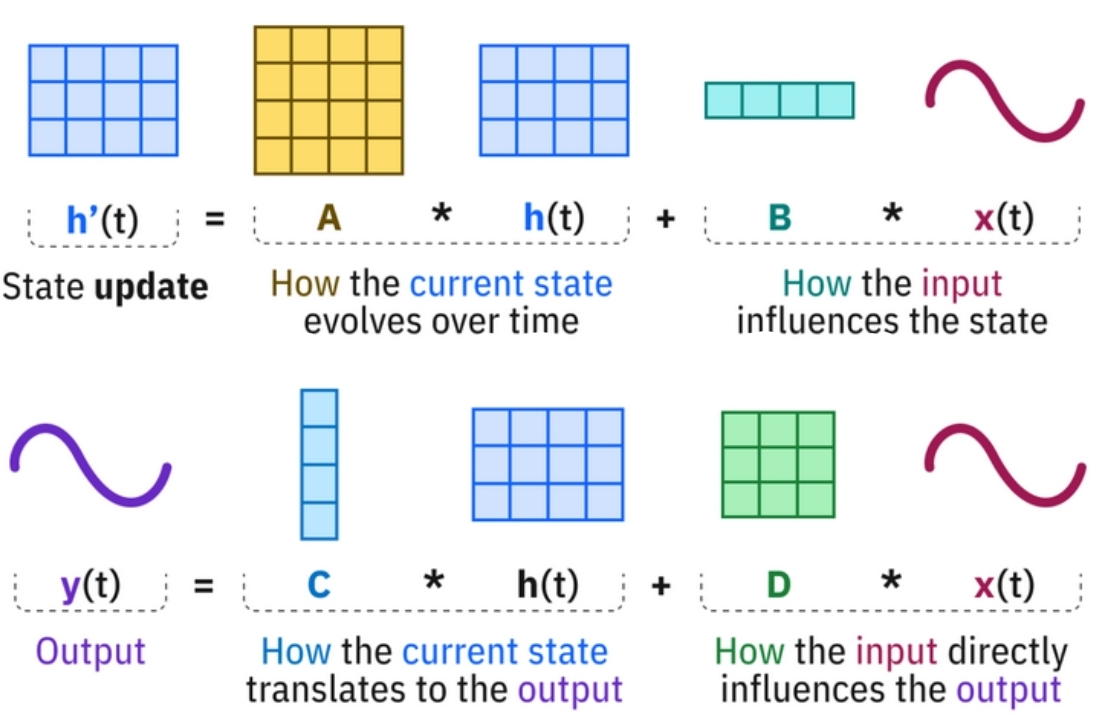
\includegraphics[width=\linewidth]{shema_matrik.png}
  \caption{Dimensions and information flow of the fitted linear state-space model. Trajectories are generated recursively with the state equation. The observation equation is included to specify the complete fitted system.}
  \label{fig:matrices}
\end{figure}

\subsection{Initial state and website production fit}

Two initial-state conditions answer RQ2. The measured-start condition uses the first state of the held-out jump. The mean-start condition averages the first states of training jumps only and recomputes that average in every fold. The same training-only rule is used for the average-path baseline. This avoids the information leakage that would occur if a single full-dataset average were reused during cross-validation.

After evaluation, a production model is fit to all 203 accepted jumps for deployment. The website asset contains a 139-sample reference profile, spanning 6.90~s from its first to last state at 0.05-s intervals. This is a control-profile length, not a training horizon: the same transition matrices are fitted to all transitions from variable-length jumps. The simulator continues beyond the reference profile when necessary to find first hill contact, up to the maximum stored sequence length of 164 samples (8.15~s), while holding the last body-control values constant. Its default initial state and control profiles are descriptive full-dataset quantities and are not used to calculate cross-validation scores.

\subsection{Cross-validation and error measures}\label{sec:evaluation}

LOOCV is performed at the jump level. For each of 203 folds, all transitions from 202 jumps are stacked to estimate the matrices, and the remaining complete jump is simulated recursively. Splitting by jump prevents transitions from the same flight from appearing in both training and test data.

Because trajectories differ in duration, we evaluate spatial rather than time-indexed separation. Each curve is sorted by longitudinal $X$, duplicate $X$ values are merged by averaging $Y$ and $Z$. Let $\mathcal{G}_i$ contain the direct pair of first points and the common integer-$X$ interpolation positions for jump $i$. After the shorter curve ends, integer-$X$ points on the longer curve and its endpoint are compared with the final point of the shorter curve. For paired points $\mathbf{p}_{ij}$ and $\widehat{\mathbf{p}}_{ij}$, the trajectory error is
\begin{equation}
E_i=\frac{1}{|\mathcal{G}_i|}\sum_{j\in\mathcal{G}_i}
\left\lVert\mathbf{p}_{ij}-\widehat{\mathbf{p}}_{ij}\right\rVert_2.
\label{eq:error}
\end{equation}
This penalizes both path separation and a prematurely ending path. The metric compares the spatial shapes of the paths, but it does not test whether the predicted jumper reaches each location at the correct time.

We additionally report three-dimensional endpoint error and terminal-coordinate-distance absolute error, where the displayed proxy is $d_{\mathrm{coord}}=\sqrt{X_{\mathrm{end}}^2+Z_{\mathrm{end}}^2}$. This is a straight-line displacement in the model coordinate system, not official hill-surface jump length. Means are accompanied by medians, sample standard deviations, maxima, and two-sided 95\% Student-$t$ confidence intervals across held-out jumps. A constant-velocity baseline extrapolates the measured initial position and velocity at 0.05~s. A fold-specific average-path baseline normalizes each training path to 1000 progress points, averages them, and restores the mean training length.

We repeat LOOCV with three predefined wind representations. The 14 states, eight speed and posture controls, measured initial state, $\alpha=10$, and fold assignments remain unchanged. The alternatives replace the 12 zone means with all 48 sensor--feature values, append squares of the 12 zone means, or use all 48 individual values and their squares. These choices produce 56, 32, and 104 controls, respectively, compared with 20 in the main model. Because the variants use the same folds and did not determine the main model, the comparison measures sensitivity to wind representation rather than independently validated performance.

\subsection{Interactive website}\label{sec:website}

The retired Shiny prototype was replaced in full by a static client-side application developed in React and TypeScript. The current website is available at \url{https://smucarski-skoki.pages.dev/}. It loads versioned JSON assets containing $A$, $B$, the baseline flight, feature order, units, default profiles, ranges, and model metadata. Simulation then runs locally in the browser, no CSV upload or server-side user-data processing is provided.

Users can apply offsets to four wind components in each of the take-off, middle, and landing zones, and to eight speed/posture profiles. The interface presents an interactive three-dimensional rendering of the sampled hill surface and simulated flight path, together with longitudinal and lateral plots and scenario presets. The rendering is implemented with Three.js, a JavaScript library that sends the scene to WebGL (Web Graphics Library), the browser's hardware-accelerated graphics interface. Three.js and WebGL affect only presentation, the state-space recurrence is calculated separately in TypeScript. Tests check matrix dimensions, exported-model parity, the first transition, finite outputs at slider extremes, and profile interpolation. Figure~\ref{fig:website} shows the new interface.

\begin{figure*}[t]
  \centering
  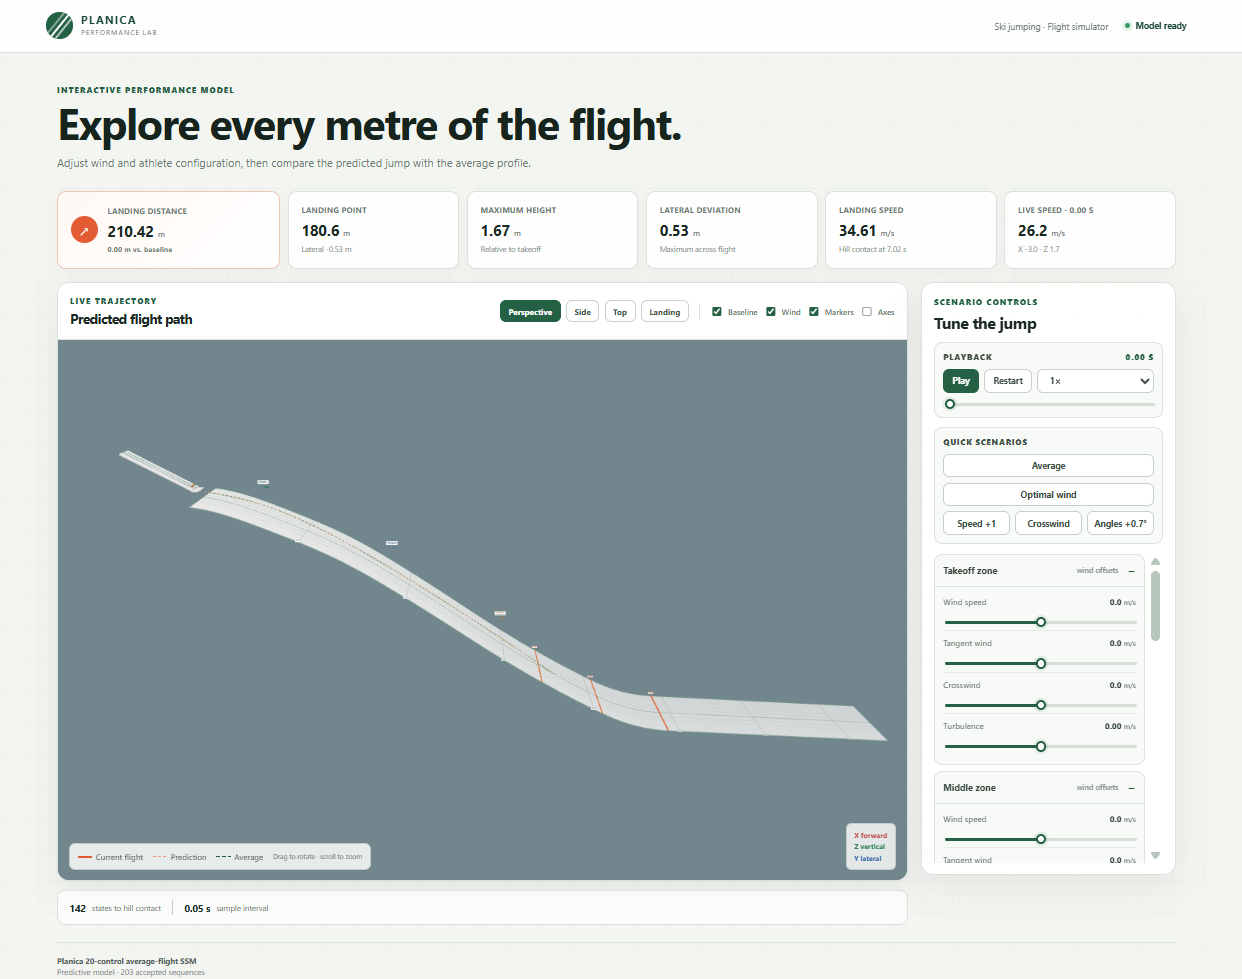
\includegraphics[width=0.96\textwidth]{website_screenshot_light.png}
  \caption{Current Ski Jump SSM Lab website. Controls on the left alter zone-wise wind and jumper-configuration profiles. The main panel displays the resulting finite-horizon path and hill geometry. The deployed page is static and executes the exported recurrence in the browser.}
  \label{fig:website}
\end{figure*}

\section{Results}\label{sec:results}

\subsection{Held-out trajectory reconstruction}

Table~\ref{tab:primary} reports LOOCV results for the fixed final model. The summary uses SD (sample standard deviation), CI, and MAE. With the measured initial state, the mean trajectory error is 1.34~m and the median is 1.18~m. Replacing it with the fold-specific mean initial state changes the mean only slightly, to 1.35~m. This result reflects the similarity of the accepted take-off states and it should not be generalized to unseen hills or athlete populations.

\begin{table}[htb]
\centering
\small
\begin{tabularx}{\columnwidth}{@{}>{\raggedright\arraybackslash}Xrrrr@{}}
\toprule
Metric (in m) & Mean & Median & SD & 95\% CI \\
\midrule
Trajectory, measured start & 1.34 & 1.18 & 0.68 & 1.24--1.43 \\
Trajectory, training-mean start & 1.35 & 1.18 & 0.69 & 1.25--1.44 \\
Endpoint, measured start & 3.55 & 3.14 & 2.04 & 3.27--3.84 \\
Terminal coordinate distance MAE & 1.68 & 1.25 & 1.83 & 1.43--1.94 \\
\bottomrule
\end{tabularx}
\caption{Held-out results across 203 LOOCV folds. SD is the sample standard deviation and CI is the two-sided Student-$t$ confidence interval for the mean. Maximum errors are 4.60, 4.70, 17.10, and 16.36~m in row order.}
\label{tab:primary}
\end{table}

The endpoint error is larger than the path-average error because recursive deviations accumulate near landing. The separate terminal-coordinate-distance MAE of 1.68~m must not be confused with the 1.34~m trajectory metric. Figure~\ref{fig:examples} shows records representative of short, typical, and long terminal-coordinate distances. To avoid selecting unusually favorable simulations, each example also lies near the median held-out trajectory error.

\begin{figure*}[t]
  \centering
  \includegraphics[width=0.95\textwidth]{revision_trajectory_representative.pdf}
  \caption{Representative measured and reconstructed trajectories under the measured-start condition. The columns jointly approximate the 10th, 50th, and 90th percentiles of measured $d_{\mathrm{coord}}$ while remaining close to the median held-out trajectory error, they are not best-case selections. The lower row exposes time-progress-aligned separation that is difficult to see at the full X--Z scale. Here $d_{\mathrm{coord}}$ is the derived coordinate displacement, not official hill-surface jump length, and $E$ is Equation~\eqref{eq:error}.}
  \label{fig:examples}
\end{figure*}

\subsection{Baselines and exploratory configurations}

The leakage-controlled average-path baseline has mean error 2.64~m (median 2.18~m, SD 2.34~m, 95\% CI 2.32--2.97~m), so the final SSM improves mean spatial error by 1.30~m on these folds. Constant-velocity extrapolation performs poorly at 58.33~m (median 59.20~m), confirming that the flight curvature cannot be represented by unforced linear motion. A physics-based or nonlinear learned baseline would provide a stronger comparison, but implementing one with matched inputs and training data remains future work.

Table~\ref{tab:windfeatures} compares four wind representations using the corrected timestamps. The 12 zone means give a mean path error of 1.339~m. Replacing them with all 48 individual sensor--feature values increases it to 1.450~m, a paired mean increase of 0.111~m (95\% CI 0.053--0.169~m). Appending the 12 squared zone-wind terms yields 1.391~m, an increase of 0.051~m (0.008--0.095~m), and combining individual values with their squares yields 1.579~m. Endpoint and terminal-coordinate-distance errors change in the same direction. Thus, under the fixed $\alpha=10$ estimator, neither retaining every sensor nor adding squared wind terms improves average held-out reconstruction. This comparison does not establish that zone averaging would remain optimal under separately tuned or independently validated models.

\begin{table*}[t]
\centering
\small
\begin{tabularx}{\textwidth}{@{}>{\raggedright\arraybackslash}Xrrrrr@{}}
\toprule
Wind representation & Controls & \shortstack{Path error\\(m)} & \shortstack{Paired path difference\\vs. zone means (95\% CI), m} & \shortstack{Endpoint error\\(m)} & \shortstack{Coordinate distance\\MAE (m)} \\
\midrule
12 zone means & 20 & 1.339 & --- & 3.555 & 1.684 \\
48 individual values & 56 & 1.450 & $+0.111$ (0.053--0.169) & 3.885 & 1.959 \\
Zone means and their squares & 32 & 1.391 & $+0.051$ (0.008--0.095) & 3.713 & 1.825 \\
Individual values and their squares & 104 & 1.579 & $+0.240$ (0.151--0.328) & 4.275 & 2.364 \\
\bottomrule
\end{tabularx}
\caption{Wind-feature sensitivity using the corrected timestamp data, the same 203 jump-level LOOCV folds, and fixed $\alpha=10$. Errors are means across held-out jumps, paired confidence intervals are two-sided Student-$t$ intervals for per-jump differences from the zone-mean model.}
\label{tab:windfeatures}
\end{table*}

A separate LOOCV check considered seven values of $\alpha$: 0.001, 0.01, 0.1, 1, 10, 100, and 1000. For the zone-mean model, mean path errors remain between 1.330 and 1.341~m through $\alpha=100$, then rise to 1.397~m at $\alpha=1000$. The lowest observed value is 1.330~m at $\alpha=100$. Thus, 10 lies on a broad performance plateau and remains a reasonable choice for the final model. The grid tests the sensitivity of the original setting, it was not used to replace that setting after examining the evaluation results. A hybrid physics-informed neural model \cite{raissi2019physics,Cai2021_PINN_FluidMechanics} was also explored but not retained because the available athlete and aerodynamic parameters were insufficient for a defensible matched implementation.

\subsection{Independent state--control sensitivity analysis}

Table~\ref{tab:independent} compares the main model with the non-overlapping formulations described in Section~\ref{sec:independent}. The seven-state, 19-control model reconstructs the overall path almost as accurately as the main model: its mean error is 1.350~m (median 1.207~m, SD 0.690~m, 95\% CI 1.254--1.445~m), compared with 1.339~m for the main model. In a paired jump-level comparison, the mean increase is only 0.010~m (95\% CI $-0.029$--0.050~m), and the independent model has the lower path error in 48.3\% of jumps. Its training-mean-start error is 1.393~m. The no-timestamp-repair subset contains 144 jumps and yields a similar mean error of 1.422~m.

\begin{table*}[t]
\centering
\small
\begin{tabularx}{\textwidth}{@{}>{\raggedright\arraybackslash}X>{\raggedright\arraybackslash}X>{\raggedright\arraybackslash}Xrrrr@{}}
\toprule
Formulation & State & Prescribed controls & Overlap & \shortstack{Path\\(m)} & \shortstack{Endpoint\\(m)} & \shortstack{Coordinate distance\\MAE (m)} \\
\midrule
Main/deployed & 14 variables & Wind, speed, posture (20) & 8 & 1.339 & 3.555 & 1.684 \\
Measured-speed diagnostic & Position and velocity (6) & Wind, speed, posture (20) & 0 & 1.340 & 3.552 & 1.663 \\
Recursive-speed independent & Position, velocity and speed (7) & Wind, posture (19) & 0 & 1.350 & 5.727 & 4.523 \\
Full-state wind-only & 14 variables & Wind (12) & 0 & 1.872 & 7.610 & 5.538 \\
No-speed kinematic & Position and velocity (6) & Wind, posture (19) & 0 & 6.808 & 33.932 & 33.350 \\
Kinematic wind-only & Position and velocity (6) & Wind (12) & 0 & 8.161 & 40.005 & 39.184 \\
\bottomrule
\end{tabularx}
\caption{Structural sensitivity results across the same 203 LOOCV folds. ``Overlap'' counts features appearing in both state and control vectors. Path is the mean of Equation~\eqref{eq:error},endpoint is mean three-dimensional endpoint error.}
\label{tab:independent}
\end{table*}

Although the mean path errors are similar, the terminal errors differ substantially. For the recursive-speed independent model, mean endpoint error is 5.727~m and terminal-coordinate-distance MAE is 4.523~m. Relative to the main model, the paired increases are 2.172~m (95\% CI 1.775--2.570~m) and 2.839~m (95\% CI 2.380--3.298~m), respectively. The independent model improves either terminal measure in only 19.7\% of jumps. Its mean spectral radius is 1.01357, so separating the vectors does not resolve finite-horizon instability.

Associations across held-out jumps are summarized using Pearson's correlation coefficient $r$, which ranges from $-1$ to $1$. Its sign indicates the direction of the linear association, while its magnitude indicates its strength. The accompanying two-sided $p$-value tests the null hypothesis of zero linear correlation. A small $p$-value provides evidence against zero correlation, but it does not measure the strength of the association and does not establish causation.

Diagnostics indicate recursive speed drift rather than a systematic directional bias. The independent model's mean speed MAE is 0.676~m/s (95\% CI 0.613--0.739~m/s). Speed MAE is strongly associated with terminal-coordinate-distance absolute error ($r=0.798$, $p<10^{-45}$), while signed terminal-speed and signed terminal-coordinate-distance errors are moderately associated ($r=0.586$, $p<10^{-19}$). Mean signed terminal-coordinate-distance error is only $-0.052$~m (95\% CI $-0.920$--0.816~m), and the mean signed $X$, $Y$, and $Z$ endpoint errors are also close to zero. Thus the degradation reflects increased between-jump dispersion and accumulated recursive error, not consistent over- or under-prediction. Flight duration is not associated with terminal-coordinate-distance absolute error ($r=0.016$, $p=0.826$), although it is moderately associated with the path metric ($r=0.309$, $p<10^{-5}$).

To determine why the recursive-speed model has much larger endpoint error despite a similar mean path error, we examined how spatial separation develops over the course of the flight. Figure~\ref{fig:independent-progress} shows how mean spatial separation changes over normalized flight progress. When measured speed is supplied at every step, separation grows from 1.52~m at 25\% progress to 3.55~m at the endpoint. Recursively predicting speed increases the corresponding values to 1.78 and 5.73~m, with the gap widening throughout the flight. These values align trajectories by flight progress and therefore differ from Equation~\eqref{eq:error}, they indicate where error accumulates.

\begin{figure}[htb]
  \centering
  \includegraphics[width=\linewidth]{independent_model_error_progression.pdf}
  \caption{Mean spatial separation at matched percentages of flight progress for two models with non-overlapping state and control variables. The seven-state model predicts speed recursively, while the six-state model receives measured speed as a control. The widening gap shows speed-related error accumulating toward the endpoint.}
  \label{fig:independent-progress}
\end{figure}

\subsection{Stability and parameter interpretation}

Across LOOCV fits, the spectral radius $\rho(A)$ has mean 1.01349, range 1.01335--1.01363, and 95\% CI 1.01349--1.01350. Because $\rho(A)>1$, the learned autonomous transition is not asymptotically stable. Simulations remain finite over the observed 4.35--8.15~s flights. The website's reference profile contains 139 states and ends at 6.90~s. If hill contact has not yet occurred, the application repeats the last available control vector and continues for at most 25 additional transitions, reaching the longest observed sequence length of 164 states or 8.15~s.

The 8.15~s limit marks the end of the observed data range, not a discontinuity in the model. The recurrence can mathematically generate further states, and a value at 8.16~s is not automatically invalid. However, the training data contain no later state transitions, LOOCV does not test them, and controls beyond 6.90~s are assumed constant rather than measured. Recursive simulation also feeds every predicted state into the next step, allowing small errors to accumulate. Moreover, a spectral radius of 1.01349 means that at least one autonomous mode grows rather than decays: repeated over the 25-step website extension, the corresponding idealized amplification is approximately $1.01349^{25}=1.40$. This is not a bound on trajectory error because the response also depends on eigenvectors, control inputs, and interactions among states, but it illustrates why apparently small per-step instability can matter under long recursion. The 8.15-s cap is therefore a validity guardrail. Longer simulation would require longer representative recordings, plausible future control profiles, external validation, and preferably stability-constrained identification.

Other entries of $A$ and $B$ are partial regression coefficients: they describe associations with the next state after accounting for the other predictors, not isolated physical effects. Because wind, posture, speed, and flight phase are correlated, ridge regression can distribute shared predictive information among several coefficients and individual signs and magnitudes may therefore change even when predictions remain similar.

Because speed and posture appear in both the state and control vectors, their separate coefficients in $A$ and $B$ are not uniquely identifiable and should not be interpreted individually. The formulations in Table~\ref{tab:independent} therefore test whether accurate reconstruction depends on this overlap.

\section{Discussion}\label{sec:discussion}

RQ1 is answered by a mean held-out spatial error of 1.34~m under measured control profiles. This shows that the regularized linear recurrence summarizes jumps from the same hill and event, within the wind, posture, speed, and trajectory ranges represented in these recordings while it does not show that the model will generalize to a different event or predict a jump from weather known before take-off. RQ2 shows little aggregate penalty from a training-only mean initial state, although both conditions still use the held-out control sequence. For RQ3, the model outperforms the two simple baselines but is not asymptotically stable. RQ4 shows that state--control overlap is not necessary for accurate average-path reconstruction: the seven-state, 19-control model obtains 1.35~m. 

The medians, standard deviations, confidence intervals, and maximum errors show variation between jumps that the mean alone would conceal. Computing the initial-state and average-path quantities from training jumps only prevents held-out data from entering either calculation. However, choices such as $\alpha$ and feature design were informed by this dataset, and the alternative formulations were not tested on new data. A separate test event, or model selection performed entirely within each training fold, would be needed for a confirmatory performance estimate. Direct numerical ranking against related works from Table~\ref{tab:related} would also be misleading because studies use different inputs and do not report Equation~\eqref{eq:error} on the same jumps.

Retaining the 14-state website model is a deployment choice, not a claim that overlapping vectors are more physically correct. The interface exposes adjustable speed and posture profiles and highlights endpoint error and the terminal coordinate-distance measure. For these outputs, the deployed model's errors of 3.55 and 1.68~m are materially lower than the recursive-speed model's 5.73 and 4.52~m. Prescribing speed also prevents its recursive error from accumulating along the longitudinal trajectory. The six-state diagnostic with measured speed performs almost identically without duplicating state variables, showing that the supplied speed profile provides the useful information. This formulation is therefore a candidate for a simpler future deployment. The website continues to describe all slider responses as conditional model associations, not causal effects.

\subsection{Limitations and scope}

The sample is small, comes from one hill and event, and lacks recoverable athlete identities and physiological covariates. Rejected files may introduce selection bias. The spatial metric does not capture timing mismatches between the measured and predicted trajectories. Fixed-interval interpolation may smooth rapid changes, while forward-filling the 21 missing roll-angle values holds the last observed angle constant across each gap. Timestamp reconstruction assumes that physical source-row order is reliable and that corrupted time values can be interpolated between trustworthy neighbors. The similar 1.39~m result in the 144-jump no-repair sensitivity analysis is reassuring, but validation against a separate record of the original measurement times would be preferable. The previous website reference profile is a separately averaged descriptive control profile and begins slightly before the take-off origin. This affects only the website's default simulation and has no effect on the cross-validation results. Unstandardized ridge regression penalizes features differently according to their units. Comparisons of the alternative model structures and the reported correlations cannot establish that speed error causes coordinate-distance error. The principal limitation is that the posture and speed profiles in the deployed model's control vector include future measurements, the independent model still uses future posture. Both are therefore conditional reconstruction and interactive response models, not causal weather-to-distance predictors.


Applying the workflow to another repeated dynamical dataset would require redefining states and controls, validating physical units, preventing group leakage, and collecting representative training sequences. This study does not establish accuracy for another hill, event, athlete group, or sport.

The website makes the fitted model inspectable but is not a validated coaching or safety system. Its static architecture removes upload and server-retention risks present in the former prototype. It still requires browser compatibility and clear communication of validity bounds.

\subsection{Future work}

Future datasets should retain an anonymized athlete identifier, cover several events and hills, and record body mass and equipment. Evaluations should select hyperparameters using training data only, scale the features, test nonlinear state-space models and matched physics baselines, and use trajectory metrics that retain timing information. Methods that constrain stability may also prevent divergence over long horizons. A model with physical constraints could keep resultant speed consistent with its velocity components, while a learned policy could replace future measured posture or speed profiles. The six-state formulation with measured speed requires prospective validation before it can replace the website model. After external validation, safety margins, hill design, wind compensation, and athlete feedback should be studied using physics-based flight simulations developed for safety and fairness \cite{muller1996dynamics}, together with trajectory-optimization methods that explicitly account for uncertainty in factors such as wind and body mass \cite{piprek2018robust}.

\section{Conclusion}\label{sec:conclusion}

We evaluated ridge-estimated linear state-space dynamics on 203 accepted Planica ski jumps. Jump-level LOOCV yields a mean conditional trajectory error of 1.34~m and a terminal-coordinate-distance MAE of 1.68~m, with substantial per-jump variation. Training-only average construction removes leakage from the evaluated initial-state and average-path conditions. A seven-state, 19-control sensitivity model with non-overlapping state and control variables retains comparable mean path accuracy of 1.35~m but increases terminal-coordinate-distance MAE to 4.52~m because speed must be propagated recursively. This distinguishes the effect of vector overlap from the value of supplying measured speed and supports retaining the current model for the website's finite-horizon terminal summaries, without implying higher physical realism. Both formulations improve on simple baselines over observed flight horizons, but their spectral radius exceed one and their measured future controls prohibit causal or long-range forecasting claims. The accompanying browser application replaces the earlier prototype and provides an accessible way to inspect bounded fitted-model responses. Proposed uses in safety, hill design, and other settings require validation on new events, hills, and athlete groups.

\subsection*{Author Contributions}
Živa Hegler is the lead author of the extended work and led the current software implementation, website, analysis, and manuscript revision. Neca Camlek contributed to earlier project. Jakob Jelenčič, Marko Grobelnik, and Dunja Mladenić contributed research guidance and manuscript review.

\subsection*{Data and Code Availability}
The source code is available in a public \href{https://github.com/zivaheg/smucarski_skoki}{GitHub repository}. It contains the timestamp repair and preprocessing code, model training and export scripts, reproducible evaluation code, and source for the client-side website. The \href{https://smucarski-skoki.pages.dev/}{interactive website} is also publicly accessible. Raw jump files cannot be redistributed because the Ski Association of Slovenia supplied them as restricted research data. The repository therefore includes analysis code and derived summaries, but not the source CSV files.

\subsection*{Acknowledgement}
{\raggedright
ARIS (Slovenian Research and Innovation Agency) supported this work through the Research Program Knowledge Technologies (grant P2-0103). European Commission support came from three Horizon Europe projects: SLAIF (Slovenian Artificial Intelligence Factory; grant 101254461), ELIAS (European Lighthouse of Artificial Intelligence for Sustainability; grant 101120237), and HumAIne (Hybrid Human--Artificial Intelligence Decision Support for Enhanced Human Empowerment in Dynamic Situations; grant 101120218). We thank the Ski Association of Slovenia for providing the ski-jump data.
\par}

\subsection*{Artificial-Intelligence-Assisted Tools}
OpenAI Codex was used during revision to assist with language editing and consistency checking. The authors reviewed the resulting text, code, and numerical outputs and remain responsible for their accuracy, originality, and interpretation.

\printbibliography[title={References}]
\end{document}
